% \documentclass[twocolumn]{aastex6}
\documentclass{aastex6}

\newcommand{\radmc}{\texttt{RADMC-3D}}
\newcommand{\kms}{ \textrm{km s}^{-1} }
\newcommand{\todo}[1]{ \textcolor{red}{#1}}
\newcommand{\vt}{ {\bm \theta}}
\newcommand{\msun}{M$_\odot$}

\shorttitle{SMA Dynamical Masses}
\shortauthors{Ian Czekala}

\begin{document}

\title{SMA Dynamical Masses}
\author{I.~Czekala\altaffilmark{1}, S.~M.~Andrews\altaffilmark{1}, D.~J.~Wilner\altaffilmark{1}, E.~L.~N.~Jensen\altaffilmark{2}, and K.~G.~Stassun\altaffilmark{3,4}}
\altaffiltext{1}{Harvard-Smithsonian Center for Astrophysics,
			 60 Garden Street, Cambridge, MA 02138; \email{iczekala@cfa.harvard.edu}}
\altaffiltext{2}{Department of Physics and Astronomy, Swarthmore College, 500 College Avenue, Swarthmore, PA 19081}
\altaffiltext{3}{Department of Physics and Astronomy, Vanderbilt University, Nashville, TN 37235}
\altaffiltext{4}{Department of Physics, Fisk University, Nashville, TN 37208}

\begin{abstract}
We present a survey of precision mass measurements for a sample of 19 well known Herbig Ae/Be and T Tauri stars. We use resolved observations with the Submillimeter Array of the Keplerian rotation of CO gas to make a precise, \emph{dynamical} mass measurement of a sample of \emph{single} stars, with 10 sources to a precision of better than 10\%. We report distance-independent quantity $M_\ast/d$ to better precision than 10\%, with distance being the main source of uncertainty, for which \emph{GAIA} will shortly ameliorate.

We use these measurements, coupled with constraints on effective temperature and luminosity, to compare to pre-main sequence model predictions in a distance-independent manner, showing that while the models do well across a variety of spectral types, there are often consistent systematic disagreements (maybe).
\end{abstract}


\section{Introduction}

Dynamical masses for all the SMA data. These sources have long been studied and are important to have accurate measurements.

Other important compilations include Hillenbrand and White, Guilloteau, Simon, Dutrey.

% Paragraph about the ability of the dynamical mass technique to measure the masses of stars.
% Tomographic reconstruction of the velocity field.
% Note the success of our groups measurements for young binaries.
% Ultimate promise is to apply this to a large measurement of single stars.
% The ultimate goal is large programs with ALMA, but there are a number of disks that have been observed with SMA for which we can already do this measurement.
We now have a technique available that delivers accurate masses \citep{rosenfeld12b, czekala15a, czekala16}.

\section{Data and Reduction}

SMA programs from which all the data was taken.

Calibration. MIRIAD software. Visibilities were exported and modeled in the UV plane.

Sources are listed in Table~\ref{table:targets}.

\begin{deluxetable*}{lccccccc}
 \tablecaption{\label{table:targets}Targets}
  \tablehead{\colhead{{Source}} & \colhead{R.A.} & \colhead{DEC} & \colhead{SPT} & \colhead{${}^{12}$CO $J$=} & \colhead{$d$ [pc]} & \colhead{Ref}}
 \startdata
LkH$\alpha$ 330 & 03:45:48.28 & +32:24:11.9 & G1--G5 & 3-2  & $315$ & ,1, \\ %schlafly14, andrews11
UX Tau A         & 04:30:04.00 & +18:13:49.4 & K1--K5 & 3-2 & $145$ & ,2, \\ %torres10, andrews11
DM Tau          & 04:33:48.72 & +18:10:09.9 & K7--M2 & 2-1 & $145$ & ,2, \\ %torres10, oberg10
AA Tau          & 04:34:55.42 & +24:28:53.2 & K6--M1 & & $145$ & ,2, \\ %torres10, andrews07
LkCa 15         & 04:39:17.80 & +22:21:03.5 & K3--K7 & 3-2 & $145$ & ,2, \\% torres10, andrews11
GM Aur          & 04:55:10.98 & +30:21:59.5 & K2--K5 & 3-2 & $145$ & ,2, \\ %torres10, hughes09
MWC 480         & 04:58:46.26 & +29:50:37.1 & A2--A8 & 2-1 & $145$ & ,2, \\ %torres10, oberg10
MWC 758         & 05:30:27.53 & +25:19:57.1 & A5--F0 & 3-2 & $279$ & ,3, \\% vanleeuwen07, isella10
CQ Tau          & 05:35:58.46 & +24:44:54.2 & F2--F6 & & $113$ & ,3, \\%vanleeuwen07, oberg10
TW Hya          & 11:01:51.91 & -34:42:17.0 & K6--M3 & 3-2 & $54$ & ,3, \\ %vanleeuwen07, andrews12
SAO 206462      & 15:15:48.44 & -37:09:16.0 &  F6--G0 & & $145$ & ,2, \\% torres10, lyo11
IM Lup          & 15:56:09.18 & -37:56:06.1 & K7--M2 & 2-1 & $155$ & ,4 \\% lombardi08, none
HD 142527       & 15:56:41.89 & -42:19:23.3 & F2--G0 & & $145$ & ,2 \\%torres10, none
RX J1604.3-2130 & 16:04:21.66 & -21:30:28.4 & K0--K3 & & $145$  & ,5, \\%dezeeuw99, mathews12
RX J1615.3-3255 & 16:15:20.23 & -32:55:05.1 & K4--K7 & 3-2 & $185$ & ,6, \\%makarov07, andrews11
RX J1633.9-2442 & 16:33:55.61 & -24:42:05.0 & K5--M0 & & $120$ & ,7, \\% loinard08, cieza12
AS 209          & 16:49:15.30 & -14:22:08.6 & K3--K6 & 3-2 & $130$ & ,3, \\%vanleeuwen07, andrews09
HD 163296       & 17:56:21.29 & -21:57:21.9 & A0--A4 & & $119$ & ,3, \\% vanleeuwen07, qi11
HD 169142       & 18:24:29.78 & -29:46:49.4 & B8--A2 & 2-1 & $145$ & ,8, \\% vanboekel05, raman08
 \enddata
 \tablecomments{References are for spectral type, distance, and previous publication of data, if exists. (1) \citet{schlafly14}, (2) \citet{torres10}, (3) \citet{vanleeuwen07}, (4) \citet{lombardi08}, (5) \citet{dezeeuw99}, (6) \citet{makarov07}, (7) \citet{loinard08}, (8) \citet{vanboekel05}}
\end{deluxetable*}

% Data Provenance
% (target, original PI, original project):
% me = Sean
%
% LkHa 330, me, Andrews et al. 2011
% UX Tau A, me, Andrews et al. 2011
% DM Tau, Karin, Oberg et al. 2010
% AA Tau, me, Andrews & Williams 2007
% LkCa 15, me, Andrews et al. 2011
% GM Aur, me, Hughes et al. 2009
% MWC 480, Karin, Oberg et al. 2010
% MWC 758, Andrea Isella, Isella et al. 2010
% CQ Tau, Karin, Oberg et al. 2010
% TW Hya, me, Andrews et al. 2012
% SAO 206462, Charlie, Lyo et al. 2011
% IM Lup, me, unpublished
% HD 142527 (not sure we'll end up using...data rough)
% RX J1604, Jonathan Williams, Mathews et al. 2012
% RX J1615, me, Andrews et al. 2011
% RX J1633, Lucas Cieza, Cieza et al. 2012 (I need to look at these data still...unsure of quality)
% AS 209, me, Andrews et al. 2009
% HD 163296, Charlie, Qi et al. 2011
% HD 169142, David, Raman et al. 2008?

\section{Methodology}

% Interferometers sample the Fourier transform of the sky brightness of the source. By forward modeling this kinematic fingerprint, we can infer parameters of the disk and precisely constrain the central stellar mass.

% Kinematic fingerprint of a molecular transition like carbon monoxide (12CO). Line transfers like CO 2-1 and 3-2, though in practice this technique is broadly applicable to a range of molecules, isotopologues, and transitions, as long as these are bright enough and distant enough in the disk to be spatially resolved.

% We use the dynamical mass technique described in \citet{czekala15a}.

% Explain how we forward model the visibilities.

% First, the goal is to create a model of the sky brightness using a physical model of the disk.

Given the diversity of disk structures, we employ several different models for the disk structure.

\subsection{Standard model}


First, create a 2D-axisymmetric model of the disk structure and velocity field, the disk model is specified in cylindrical coordinates. This is informed by stellar mass $M_\ast$, a power law temperature distribution with normalization at 10 AU $T_{10}$ and gradient $q$.

Vertically isothermal disk.

\begin{equation}
	T(r) = T_{10} \left ( \frac{r}{\textrm{10 AU}}\right)^{-q}
\end{equation}

\citet{rosenfeld13a} have shown that terms like vertical geometry, disk-self gravity, and radial pressure gradient amount to small contributions on the mass inference.

Surface density profile, set with $\gamma = 1$. The normalization of this profile is given by the pre-factor $\Sigma_c$, and the total disk mass ($M_\textrm{disk}$) can be found by integrating $\Sigma(r)$ over the surface area of the disk.

\begin{equation}
\Sigma(r) = \Sigma_c \left (\frac{r}{r_c} \right)^{- \gamma} \exp \left[ - \left(\frac{r}{r_c} \right)^{2 - \gamma} \right]
\end{equation}

The disk is assumed to be in hydrostatic equilibrium, and so the gas density structure is given by
\begin{equation}
\rho(r, z) = \frac{\Sigma(r)}{\sqrt{2 \pi} H} \exp \left [- \frac{z^2}{2 H^2} \right]
\end{equation}

where the scale height $H$ is given by

\subsection{Cavity model}

With respect to the standard model, the cavity model is modified by an inner exponential taper, with location $r_\textrm{cav}$ and gradient $\gamma_c$

\begin{equation}
\Sigma(r) = \Sigma_c \left (\frac{r}{r_c} \right)^{- \gamma} \exp \left [- \left ( \frac{r_\mathrm{cav}}{r} \right)^{\gamma_c} \right ]  \exp \left[ - \left(\frac{r}{r_c} \right)^{2 - \gamma} \right]
\end{equation}

We elect to use a model with a smooth transition over more conventional models of gas cavities, such as a simple depletion factor inside some radius) because of the finite grid used to do the radiative transfer. It is necessary to ``resolve'' the transition in the radiative transfer to reduce the entrance of numerical artifacts, and this is impossible to do with a model with a sharp transition.

We set a prior that $r_\textrm{cav} \leq r_c$ and $\gamma_c \geq 0$.

Then, this structure is ray-traced using the radiative transfer program \texttt{RADMC-3D}, whereby disk orientation effects such as disk inclination $i_d$ and position angle $\varphi$ are taken into account. Disk inclination is defined using the orientation of the disk angular momentum vector from the line of sight to the observer. 0\degr is a face-on disk with the vector pointed towards the observer, 90\degr is an edge-on disk, and 180\degr is a face-on disk with the vector pointed away from the observer. We enforce a geometrical prior on the inclination of the disk, $p(i_d) =  \sin(i_d)/2$, designed to account for the fact that a disk is more likely to be observed edge-on than face-on.

Likewise, position angle is defined using the projection of the disk angular momentum vector on the plane of the sky, in degrees running East of North (counter clockwise on the sky).

The angular scale of the disk are set according to the distance $d$ to the source, which generally factors into a linear dependence on the mass uncertainty. Stellar mass is generally uncorrelated with other parameters. With corrections for phase center offsets $\mu_\alpha$ and $\mu_\delta$.


% Two dimensional, axi-symmetric convention.

Inclination convention. Position angle convention. Notes on geometrical prior.

Explore this posterior with MCMC on a cluster. After running multiple chains to asses convergence, burn-in is removed and posteriors are calculated. A full example of the 12-dimensional posterior is shown in Figure~\ref{fig:posterior}.

The sources are fit with a fixed distance. Including distance floating \citep[e.g.,][]{czekala15a,czekala16} simply creates a linear mass degeneracy, with minor changes to disk size and mass. This posterior is folded in to the mass uncertainty in a linear manner.

\footnote{We have released this dynamical mass code as a publicly available, open-source (under an MIT liscence) package written in the \texttt{Julia} language, available at \url{https://github.com/iancze/DiskJockey}}

\section{Results}

We present our results in Table~\ref{table:masses}.

We present a table of the model parameters shared by each model, and list the evaluations done by each model in the table. As you can see, there are minimal changes in stellar mass.

Note that because the disk structures are derived from optically thick transitions, we caution about the interpretability of the disk structure itself, particularly inference about the total disk mass. Previous fits using these transitions have been shown to yield accurate stellar masses, and $M_\ast$ in generally is rather insensitive to small inaccuracies in disk structure. In essentially, these disk structure parameters are carted around as nuisance parameters to fit the disk.

% I think an interesting figure for this section would be to plot a representative set of PMS tracks (Dartmouth), then plot the existing disk-based sources in transparent blue, plot the existing eclipsing binary sources in transparent red, then plot our updated disk based measurements in a bold blue. Below, we will have a histogram showing where these have been filled in.

% Stars that are in Tycho-2 catalog, and will presumably have astrometric solutions from the first GAIA release, on September 14th.
% LkHa 330
% UX Tau A
% LkCa 15
% GM Aur
% MWC 480
% MWC 758
% CQ Tau
% TW Hya
% SAO 206462
% HD 142527
% AS 209
% HD 163296
% HD 169142
% that's 13 / 19 sources, which is excellent.

% Data Provenance
% (target, original PI, original project):
% me = Sean
%
% LkHa 330, me, Andrews et al. 2011
% UX Tau A, me, Andrews et al. 2011
% DM Tau, Karin, Oberg et al. 2010
% AA Tau, me, Andrews & Williams 2007
% LkCa 15, me, Andrews et al. 2011
% GM Aur, me, Hughes et al. 2009
% MWC 480, Karin, Oberg et al. 2010
% MWC 758, Andrea Isella, Isella et al. 2010
% CQ Tau, Karin, Oberg et al. 2010
% TW Hya, me, Andrews et al. 2012
% SAO 206462, Charlie, Lyo et al. 2011
% IM Lup, me, unpublished
% HD 142527 (not sure we'll end up using...data rough)
% RX J1604, Jonathan Williams, Mathews et al. 2012
% RX J1615, me, Andrews et al. 2011
% RX J1633, Lucas Cieza, Cieza et al. 2012 (I need to look at these data still...unsure of quality)
% AS 209, me, Andrews et al. 2009
% HD 163296, Charlie, Qi et al. 2011
% HD 169142, David, Raman et al. 2008?

\begin{deluxetable*}{lcccccccccccc}
 \tablecaption{\label{table:masses}Inferred System Properties}
  \tablehead{\colhead{{Source}} & \colhead{$M_\ast$} & \colhead{$i_d$} & \colhead{$r_c$} & \colhead{$\log M_\textrm{CO}$} & \colhead{$T_{10}$} & \colhead{$q$} & \colhead{$\xi$} & \colhead{P.A.} & \colhead{$r_\mathrm{cav}$} & \colhead{$\gamma_\mathrm{cav}$} \\
	& \colhead{[$M_\odot$]} & \colhead{[${}^\circ$]} & \colhead{[AU]} & \colhead{[$M_\odot$]} & \colhead{[K]} & & \colhead{ [$\kms$]} & \colhead{[${}^\circ$]} & \colhead{[AU]} & }
 \startdata
 LkH$\alpha$ 330 & \\
 UX Tau A & \\
 DM Tau & \\
 AA Tau & \\
 LkCa 15 & $1.11_{-0.18}^{+0.09}$ & $45.7_{-2.3}^{+1.1}$ & $470_{-131}^{+105}$ & $-3.9_{-0.2}^{+0.2}$ & $94_{-14}^{+6}$ & $0.57_{-0.04}^{+0.02}$ & $0.48_{-0.05}^{+0.02}$ & $153.2_{-1.0}^{+1.0}$  \\
 GM Aur & \\
 MWC 480 & $2.14_{-0.51}^{+0.22}$ & $35.2_{-1.4}^{+0.4}$ & $136_{-21}^{+45}$ & $-3.7_{-0.1}^{+0.1}$ & $325_{-39}^{+29}$ & $0.75_{-0.01}^{+0.02}$ & $0.29_{-0.01}^{+0.01}$ & $58.4_{-0.2}^{+0.4}$ \\
 MWC 758 & \\
 CQ Tau & \\
 TW Hya & \\
 SAO 206462 & \\
 IM Lup & \\
 HD 142527 & \\
 RX J1604 & \\
 RX J1615 & \\
 RX J1633 & \\
 AS 209 & \\
 HD 163296 & \\
 HD 169142 & \\
% LkH$\alpha$ 330 & \tablenotemark{a}  \\
% UX Tau A         &\\
% DM Tau          & \\
% AA Tau          & \\
% LkCa 15         & \\
% GM Aur          & \\
% MWC 480         & \\
% MWC 758         & \\
% CQ Tau          & \\
% TW Hya          & \\
% SAO 206462      & \\
% IM Lup          & \\
% HD 142527       & \\
% RX J1604 				& \\
% RX J1615 				& \\
% RX J1633 				& \\
% AS 209          & \\
% HD 163296       & \\
% HD 169142       & \\
 \enddata
 \tablenotetext{a}{From lack of sufficient sensitivity in the channels at the systemic velocity or any external constraints, it is unknown whether the absolute orientation of the disk inclination vector is pointed towards ($0\degr \leq i_d \leq 90\degr$) or away from ($90\degr \leq i_d \leq 180\degr$) the observer.}
 \tablecomments{Full posterior and likelihood samples are provided for download \todo{at figshare HERE.}}
\end{deluxetable*}

\begin{figure*}[htb]
\begin{center}
  \includegraphics[draft,width=0.95\textwidth,height=7in]{posterior_example.pdf}
  \figcaption{
  A giant, 12 parameter figure showing the full parameter space. Explaining the various parameters and how they are connected. Note that a 13th parameter $M_\ast / d$ has been computed from the samples of $M_\ast$ and $d$ and is not sampled directly.
  \label{fig:posterior}}
  \end{center}
\end{figure*}

\begin{figure*}[htb]
\begin{center}
\includegraphics[draft, width=2.3in, height=2.15in]{LkHa330_posterior.pdf}
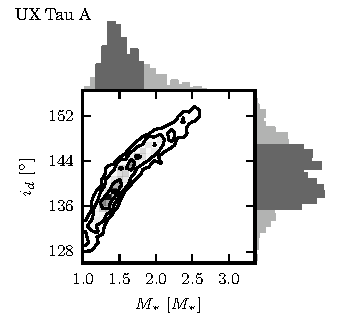
\includegraphics{UXTauA_posterior.pdf}
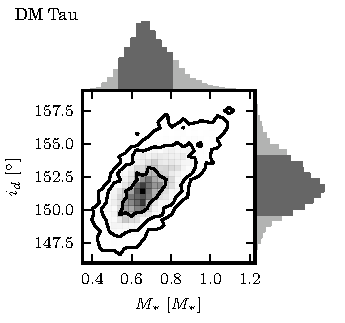
\includegraphics{DMTau_posterior.pdf}
\includegraphics[draft, width=2.3in, height=2.15in]{AATau_posterior.pdf}
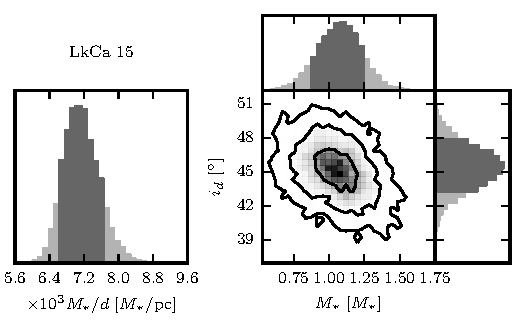
\includegraphics{LkCa15_posterior.pdf}
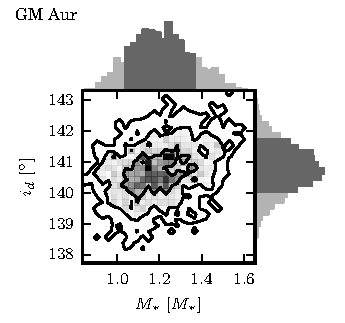
\includegraphics{GMAur_posterior.pdf}
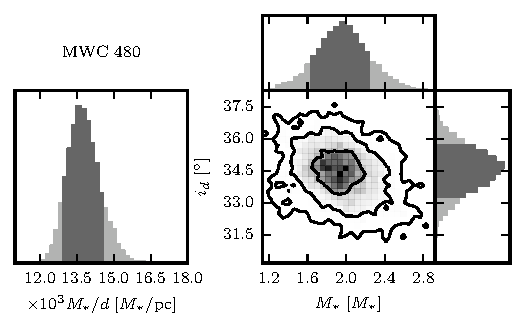
\includegraphics{MWC480_posterior.pdf}
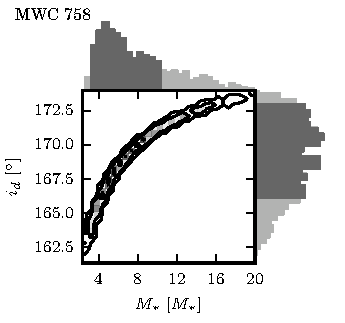
\includegraphics{MWC758_posterior.pdf}
\includegraphics[draft, width=2.3in, height=2.15in]{CQTau_posterior.pdf}
\figcaption{All of the tiny posteriors.
\label{fig:posteriors_one}
}
\end{center}
\end{figure*}

\begin{figure*}[htb]
\begin{center}
\includegraphics[draft, width=2.3in, height=2.15in]{TWHya_posterior.pdf}
\includegraphics[draft, width=2.3in, height=2.15in]{SAO206462_posterior.pdf}
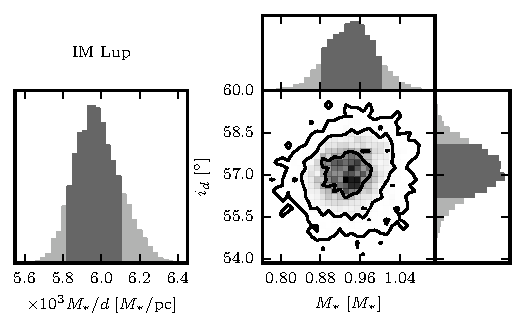
\includegraphics{IMLup_posterior.pdf}
\includegraphics[draft, width=2.3in, height=2.15in]{HD142527_posterior.pdf}
\includegraphics[draft, width=2.3in, height=2.15in]{RXJ1604_posterior.pdf}
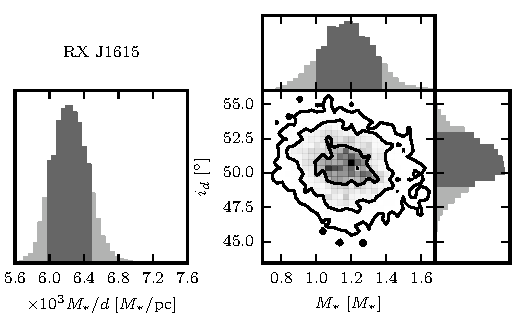
\includegraphics{RXJ1615_posterior.pdf}
\includegraphics[draft, width=2.3in, height=2.15in]{RXJ1633_posterior.pdf}
\includegraphics[draft, width=2.3in, height=2.15in]{AS209_posterior.pdf}
\includegraphics[draft, width=2.3in, height=2.15in]{HD163296_posterior.pdf}
\figcaption{All of the tiny posteriors.
\label{fig:posteriors_two}
}
\end{center}
\end{figure*}

\begin{figure}[htb]
\begin{center}
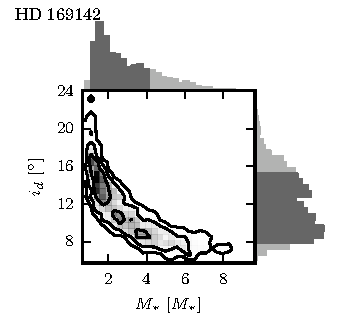
\includegraphics{HD169142_posterior.pdf}
\figcaption{All of the tiny posteriors.
\label{fig:posteriors_three}
}
\end{center}
\end{figure}

\subsection{Comparison to pre-main sequence evolutionary models}

We use literature values for the estimate of spectral type, effective temperature, and luminosity to place these sources on the pre-main sequence Hertzsprung Russel sp? (HR) diagram. We use a selection of pre-main sequence models from the X, Y, and Z. And we color-code the discrepancy between our measurement and the predicted mass from the photospheric properties.

\begin{figure*}[htb]
\begin{center}
  \includegraphics[draft,width=\textwidth,height=0.5\textheight]{PMS.pdf}
  \figcaption{
  PMS comparison HR diagram, showing probability of agreement as color coded circle.
  \label{fig:PMS}}
  \end{center}
\end{figure*}


\section{Conclusions}

We present the largest compilation of disk-based dynamical mass measurements to date.

We find that the pre-main sequence models (do not) work for X, Y, and Z.

\acknowledgments
IC is supported by the Smithsonian Institution. The authors would like to acknowledge Adam Kraus for helpful discussions regarding the distance to LkH$\alpha$~330; Jane Huang for helpful conversations about the cloud contamination of AS~209. \todo{SA acknowledges XX}. \todo{SMA observers of this data?}  Figures \todo{XX} were generated with \texttt{triangle.py} \citep{foreman-mackey14}. This research made extensive use of the Julia programming language \citep{julia12} and Astropy \citep{astropy13}.

\software{Julia, \citep{julia12}}

\bibliographystyle{yahapj.bst}
\bibliography{SMA.bib}

\appendix

\section{Remarks on individual sources}

\subsection{LkH$\alpha$ 330}
\begin{figure*}[htb]
\begin{center}
  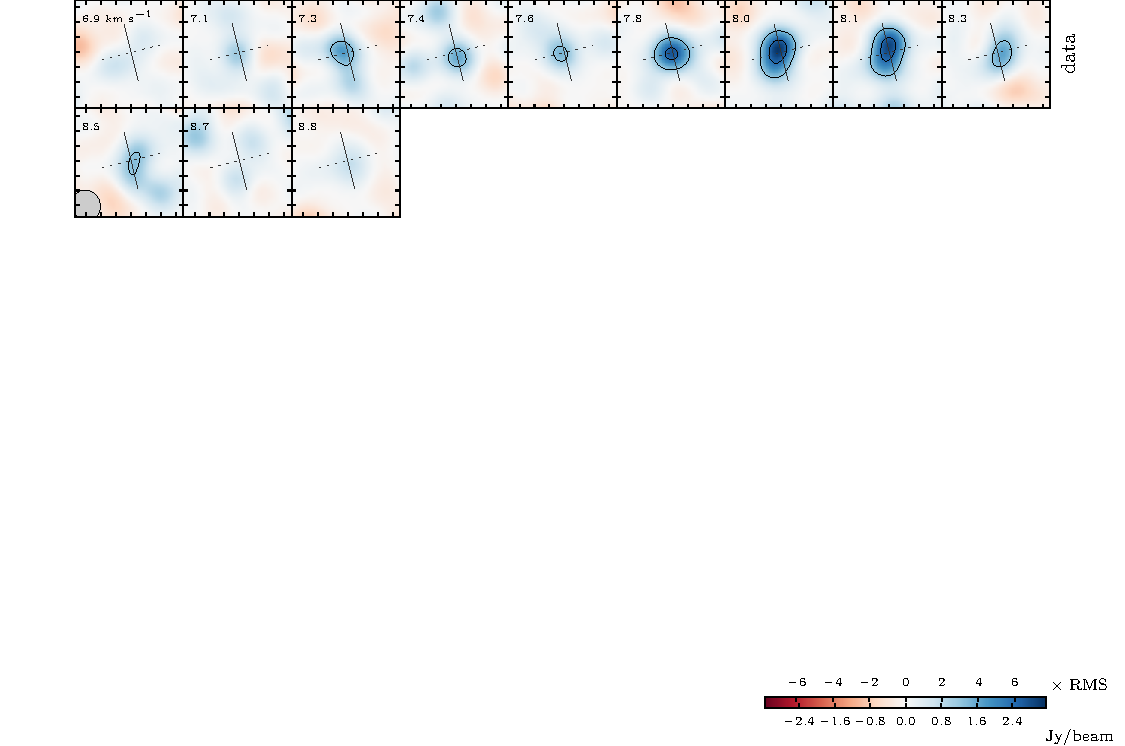
\includegraphics{LkHa330.pdf}
  \figcaption{
  Model, data, and residual channel maps for LkHa~330. Contours are every 3 sigma. Negative residuals are denoted by dashed contours. Color bar labels intensity in multiples of the RMS as well as Jy/beam.
  \label{fig:LkHa330}}
  \end{center}
\end{figure*}

\citet{isella13} find azimuthal asymmetry in the dust ring. Dynamical interactions by unseen low mass planets.
\citep{andrews11a} find the following parameters:
\citep{pontoppidan11} use CRIRES. Shows narrow, blended peak characteristic of a face-on disk at 9 kms LSR. Assuming M=2.5, they derive i = 12, however these are clearly degenerate. For M = 1.6, 17 degrees. If our results are funky, this might be nice to combine as well.

PA=218. CO v = 1 - 0.

% Andrews et al. 2011 determine the following parameters from dust + photometry
% SPT = G3.
% dpc = 250 pre
% M = 2.5 sun.
% i = 35 deg.
% r > 130 AU.
% Dust cavity of 40 AU.

% Strangely, gas modeling does NOT support this mass and inclination combination.

\subsection{UX Tau A}

Although it looks good in the channel maps, this fit is clearly wrong. The disk does not contain $10^5 M_odot$ of material.

\begin{figure*}[htb]
\begin{center}
  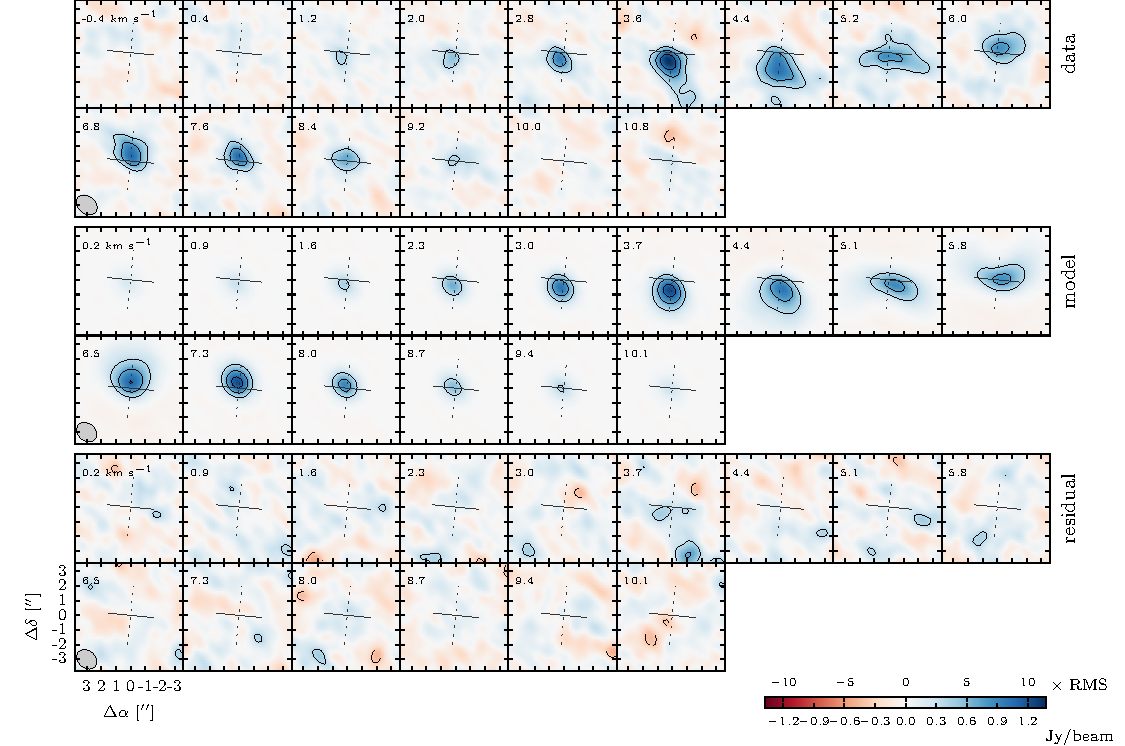
\includegraphics{UXTauA.pdf}
  \figcaption{
  Same as above, for UX~Tau~A.
  \label{fig:UXTauA}}
  \end{center}
\end{figure*}

\citep{espaillat07}.

\citet{tanii12} say west side is nearest, so we use negative inclination.

% i = 46 +/- 2
% west side nearest
% no evidence of a gap up to 20 AU.

\subsection{DM Tau}
Previous measurements.

Dartois 03 paper CO channel maps (at higher spatial and velocity resolution) suggest that the inclination is > 90 degrees. Subsequent analysis (Teague, Loomis) assume ~35 degrees inclination and make no attempt to disambiguate absolute orientation of inclination.

\begin{figure*}[htb]
\begin{center}
  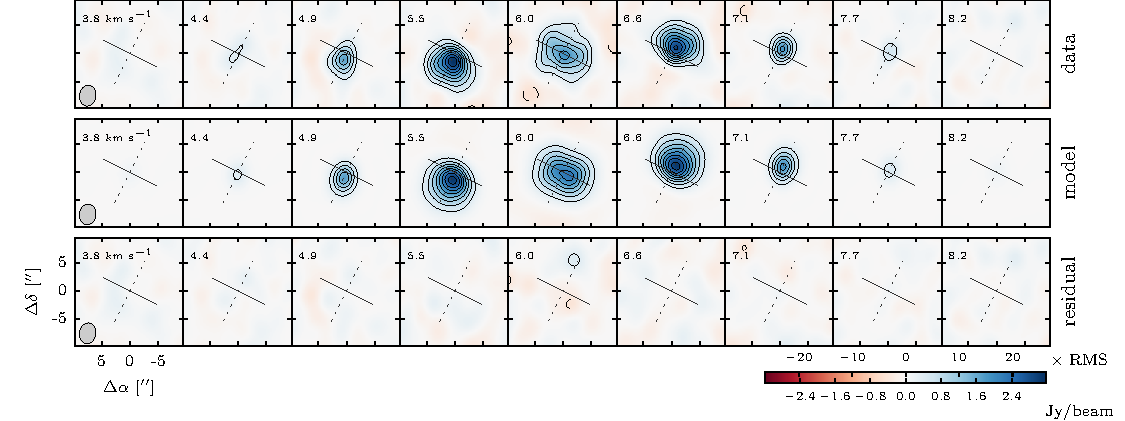
\includegraphics{DMTau.pdf}
  \figcaption{
  Same as above, for DM~Tau.
  \label{fig:DMTau}}
  \end{center}
\end{figure*}

\subsection{AA Tau}

\begin{figure*}[htb]
\begin{center}
  \includegraphics[draft, width=0.95\textwidth, height=5in]{AATau.pdf}
  \figcaption{
  Same as above, for AA~Tau
  \label{fig:AATau}}
  \end{center}
\end{figure*}

\subsection{LkCa 15}
Previous measurements. Transition disk.

\citep{vandermarel15} notes PA = 60 deg, i = 55 deg,  vsrc=6.1.

What do we say about the presence of a gap?

\begin{figure*}[htb]
\begin{center}
  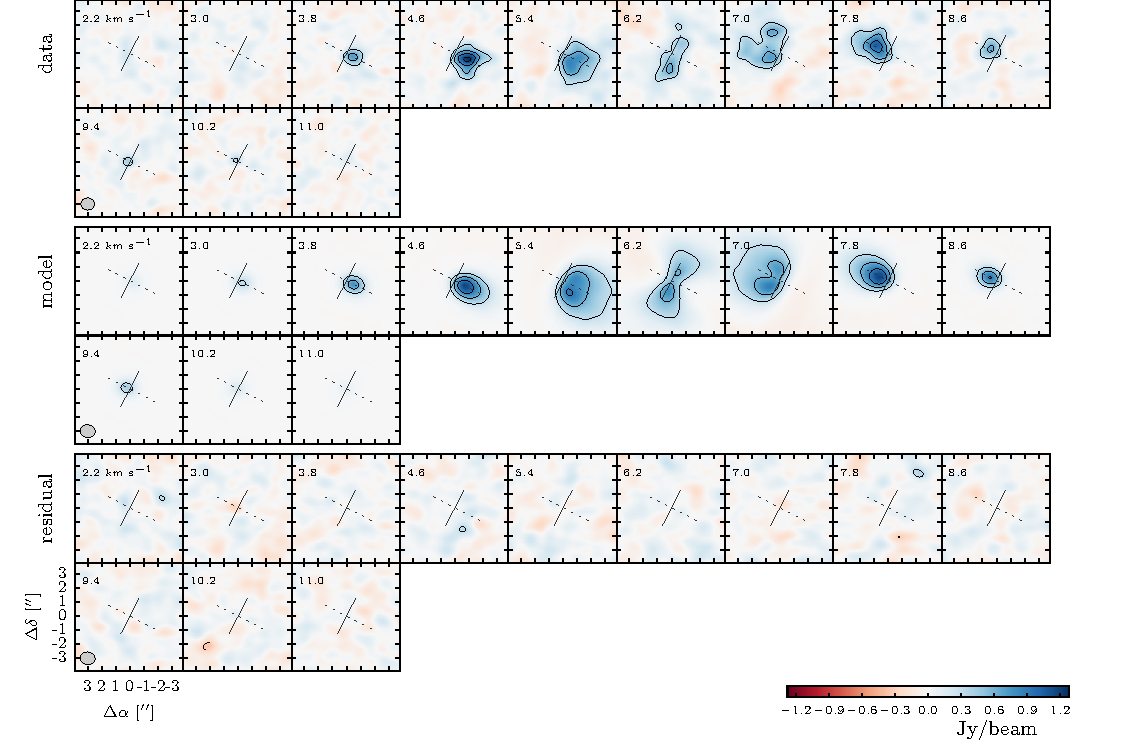
\includegraphics{LkCa15.pdf}
  \figcaption{
  Same as above, for LkCa~15.
  \label{fig:LkCa15}}
  \end{center}
\end{figure*}

\subsection{GM Aur}
Previous measurements.

\begin{figure*}[htb]
\begin{center}
  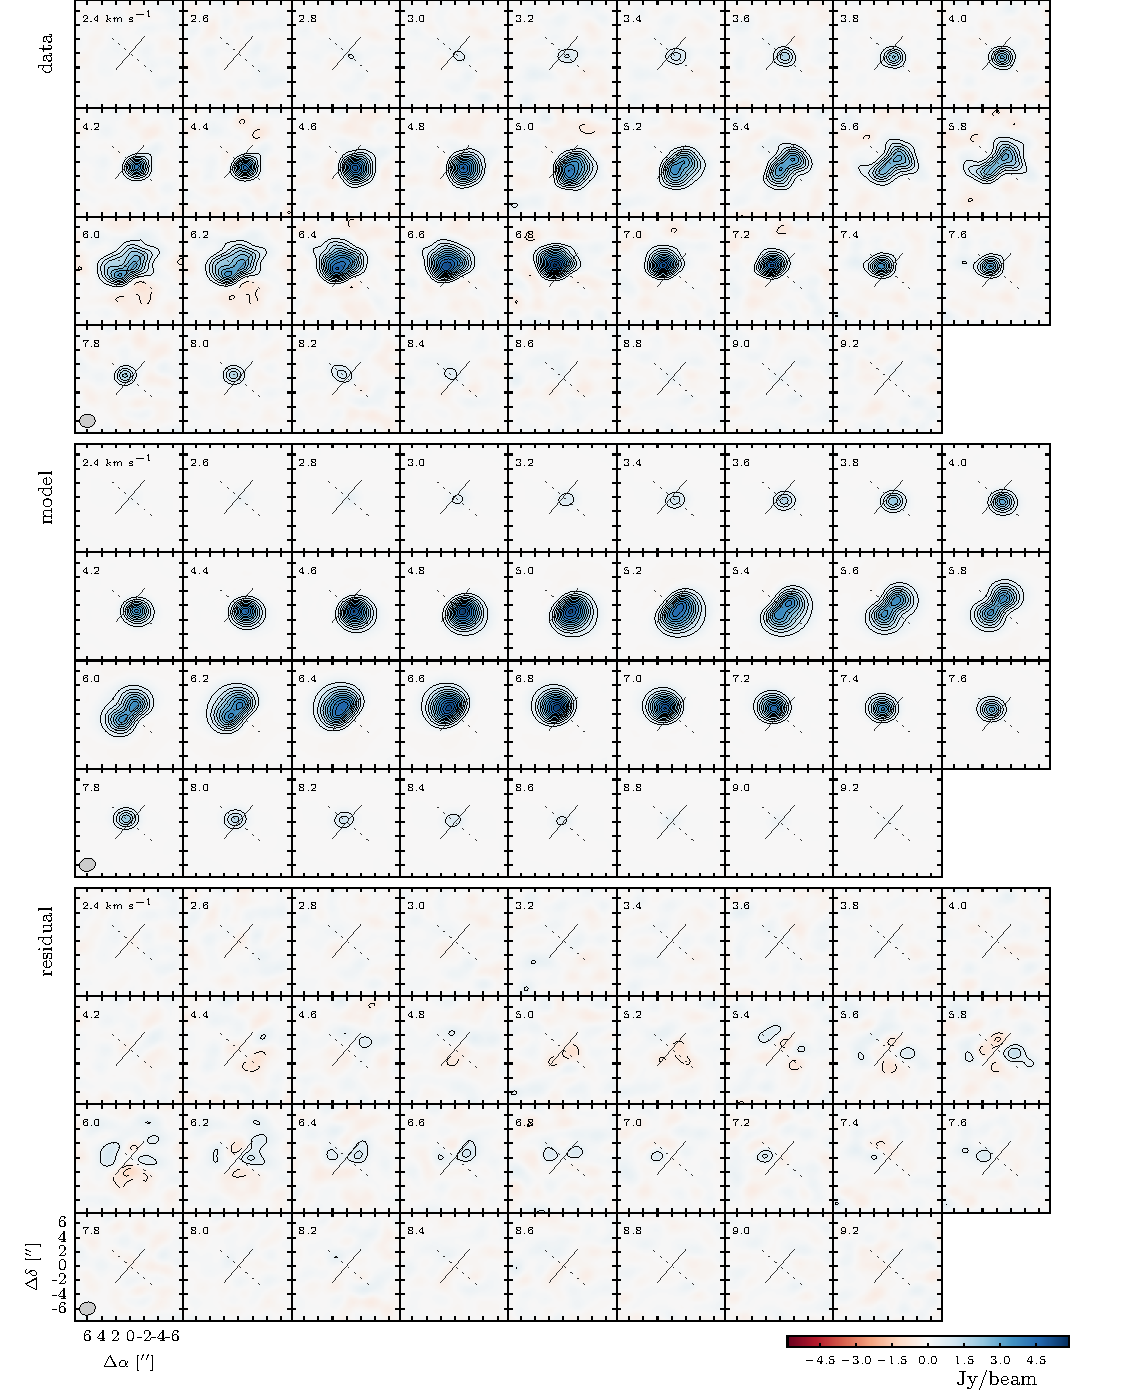
\includegraphics{GMAur.pdf}
  \figcaption{
  Same as above, for GM~Aur.
  \label{fig:GMAur}}
  \end{center}
\end{figure*}


\subsection{MWC 480}
\begin{figure*}[htb]
\begin{center}
  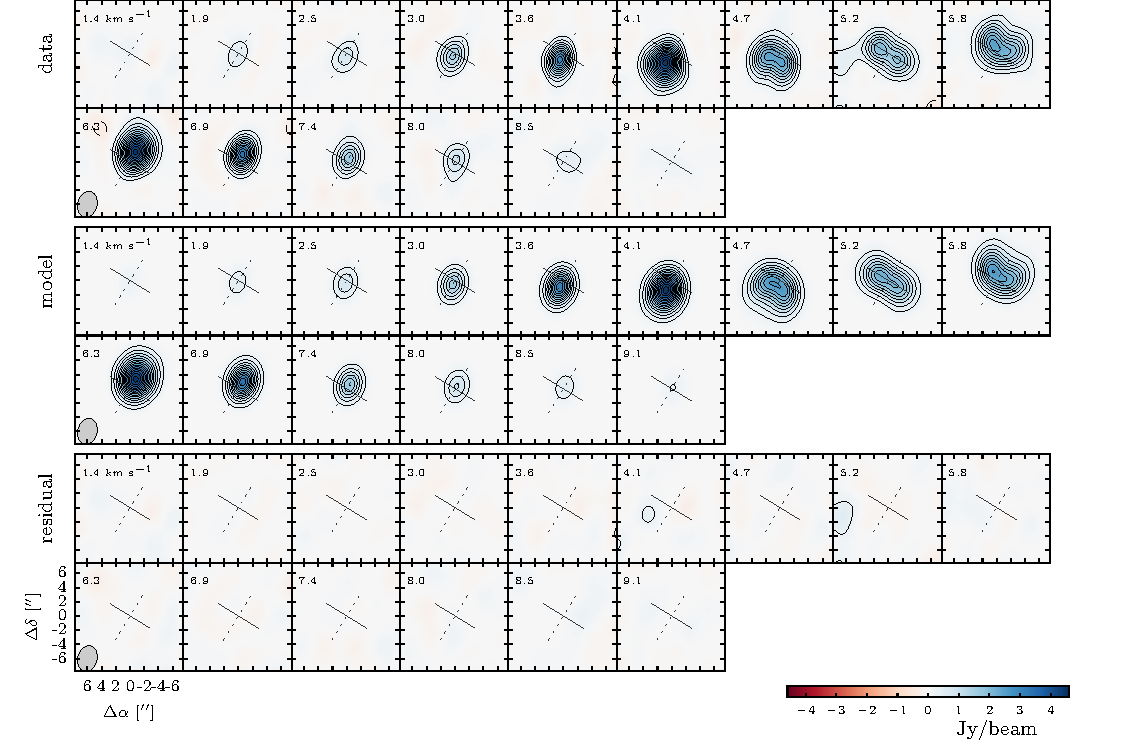
\includegraphics{MWC480.pdf}
  \figcaption{
  Same as above, for MWC~480.
  \label{fig:MWC480}}
  \end{center}
\end{figure*}

\subsection{MWC 758}

\begin{figure*}[htb]
\begin{center}
  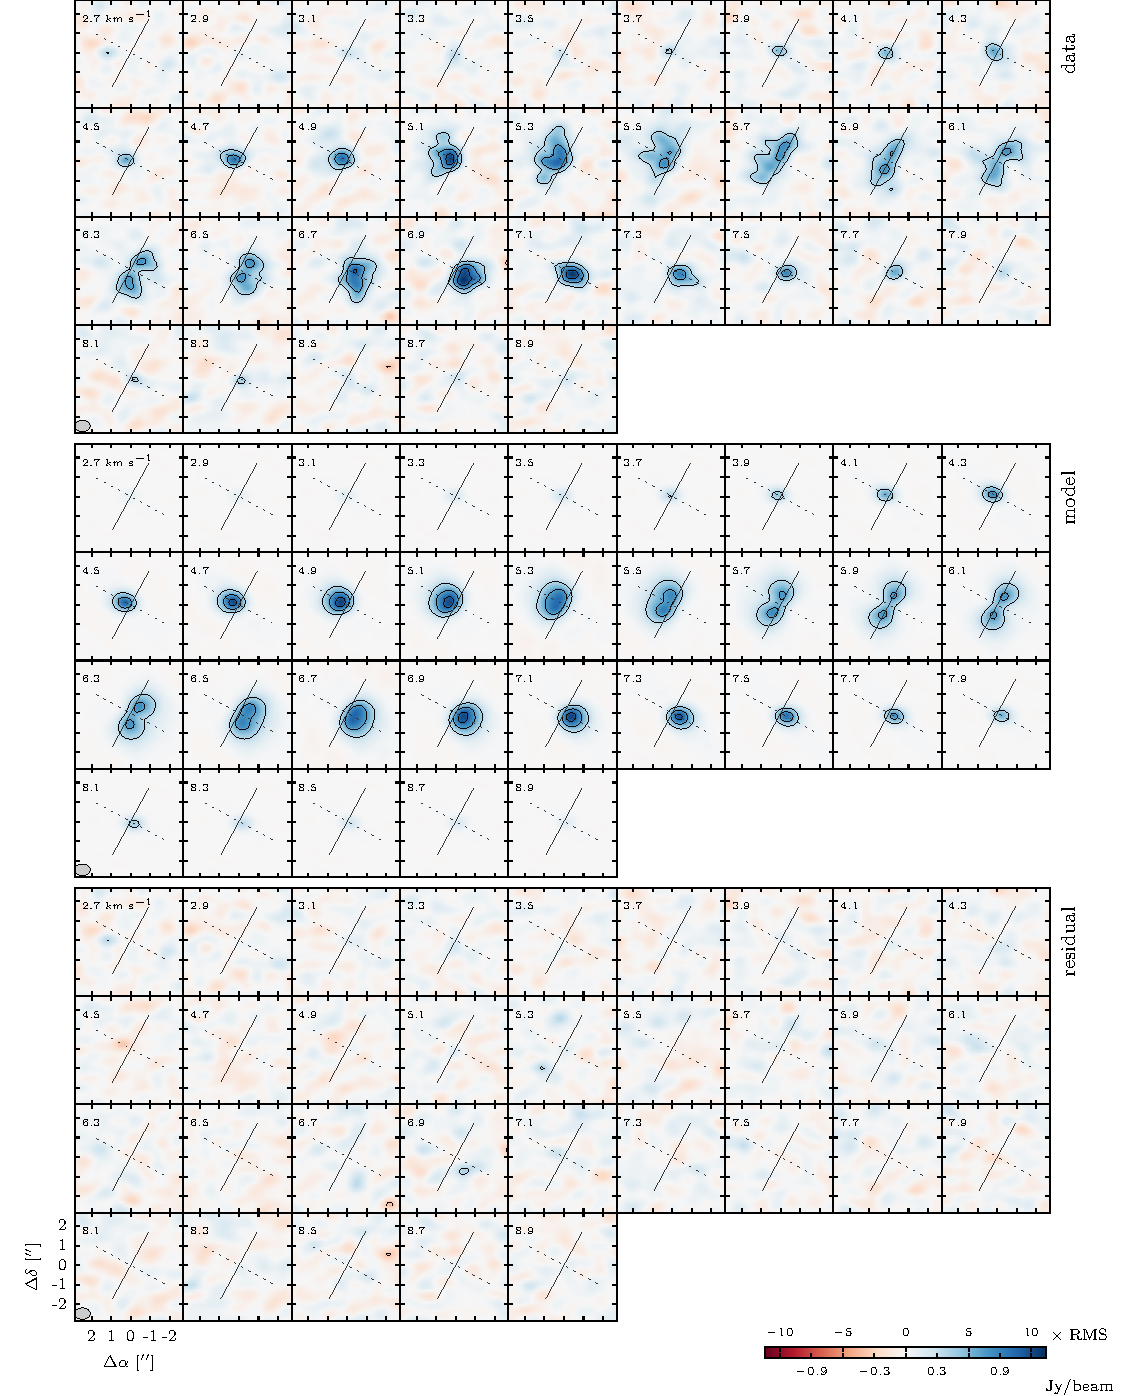
\includegraphics{MWC758.pdf}
  \figcaption{
  Same as above, for MWC~758.
  \label{fig:MWC758}}
  \end{center}
\end{figure*}

\subsection{CQ Tau}
% Parallax from van Leeuwen
% 8.85 [1.80]

\begin{figure*}[htb]
\begin{center}
  \includegraphics[draft, width=0.95\textwidth, height=5in]{CQTau.pdf}
  \figcaption{
  Same as above, for CQ~Tau.
  \label{fig:CQTau}}
  \end{center}
\end{figure*}

\subsection{TW Hya}

\begin{figure*}[htb]
\begin{center}
  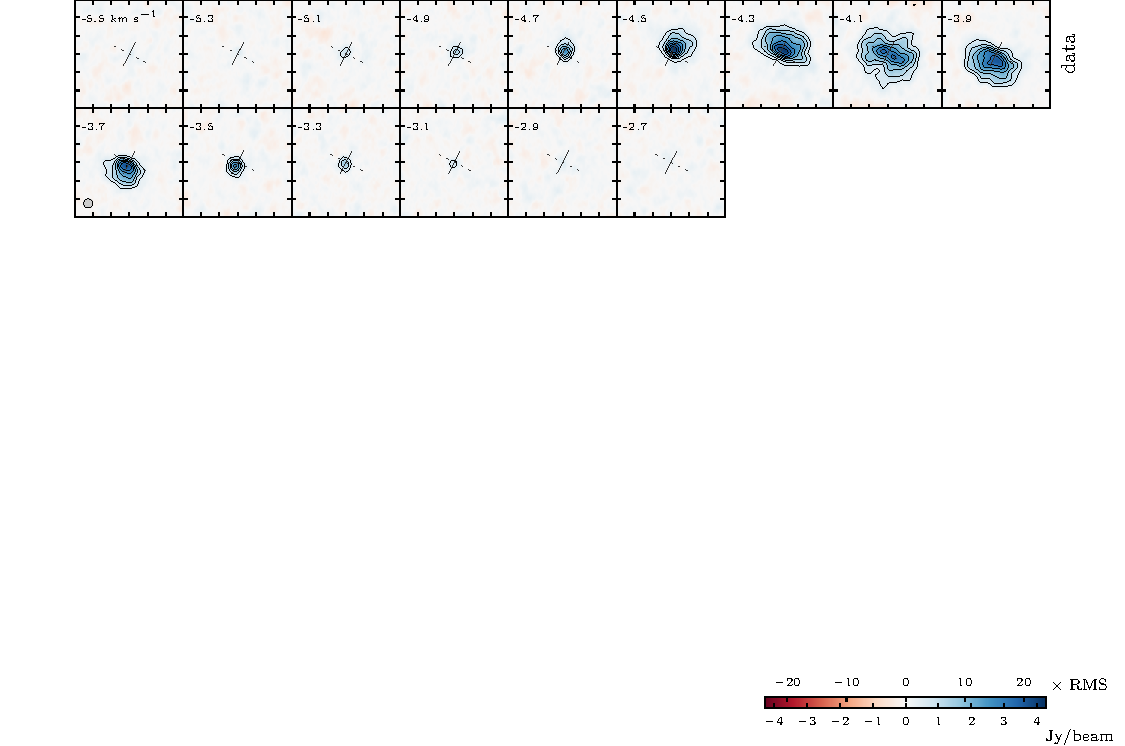
\includegraphics{TWHya.pdf}
  \figcaption{
  Same as above, for TW~Hya.
  \label{fig:TWHya}}
  \end{center}
\end{figure*}

\subsection{SAO 206462}

\begin{figure*}[htb]
\begin{center}
  \includegraphics[draft, width=0.95\textwidth, height=5in]{SAO206462.pdf}
  \figcaption{
  Same as above, for SAO~206462.
  \label{fig:SAO206462}}
  \end{center}
\end{figure*}

\subsection{IM Lup}

Galli and Bertout quote the SPM4 (Girard et al 2011) catalog for a parallax of 5.3 +/- 1.4 milliarcseconds.

I convert this to 188.7 +/-
149.3 to 256.4

- 40pc + 67 pc

\begin{figure*}[htb]
\begin{center}
  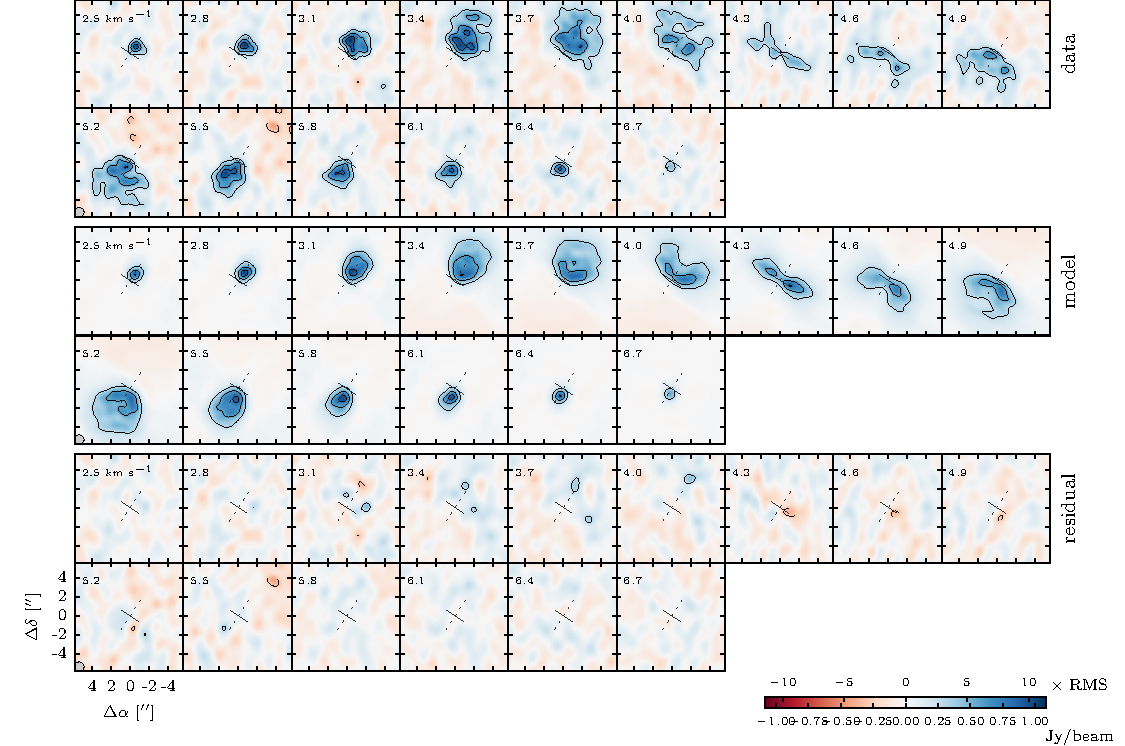
\includegraphics{IMLup.pdf}
  \figcaption{
  Same as above, for IM~Lup.
  \label{fig:IMLup}}
  \end{center}
\end{figure*}

\subsection{HD 142527}

% To watch out for? https://public.nrao.edu/news/pressreleases/binary-star-disk

% M dwarf star is in the transition disk: \url{http://arxiv.org/abs/1511.09390}

% Model the Hercshel data. http://arxiv.org/abs/1606.07266

\begin{figure*}[htb]
\begin{center}
  \includegraphics[draft, width=0.95\textwidth, height=5in]{HD142527.pdf}
  \figcaption{
  Same as above, for HD~142527.
  \label{fig:HD142527}}
  \end{center}
\end{figure*}

\subsection{RX J1604.3-2130}

\begin{figure*}[htb]
\begin{center}
  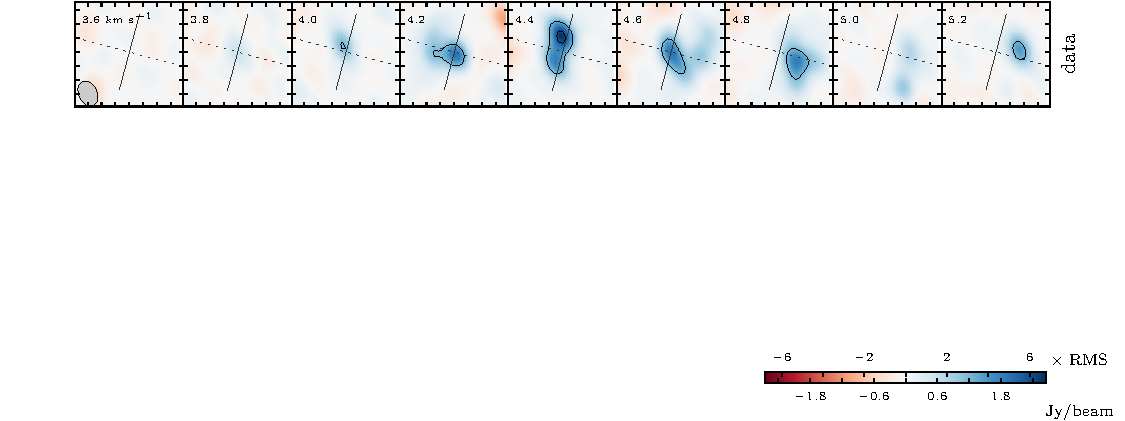
\includegraphics{RXJ1604.pdf}
  \figcaption{
  Same as above, for RX J1604.3-2130.
  \label{fig:RXJ1604}}
  \end{center}
\end{figure*}

\citep{vandermarel15} notes that this is viewed almost face-on (Mathews 12, Zhang 14). PA = 80, i = 10, vsrc = 4.7 km/s.

Dahm 08, Mathews 12, Carpenter 14

$M = 1.0 M_\odot$.
Spt = K2
d = 145 pc

Dust shadowing by an inner disk. A ``double drop'' going on at two radii.

Gas density drop at 30 AU.

% VLT/Sphere Also see a 30 AU cavity. http://arxiv.org/abs/1606.07087

\subsection{RX J1615.3-3255}
\begin{figure*}[htb]
\begin{center}
  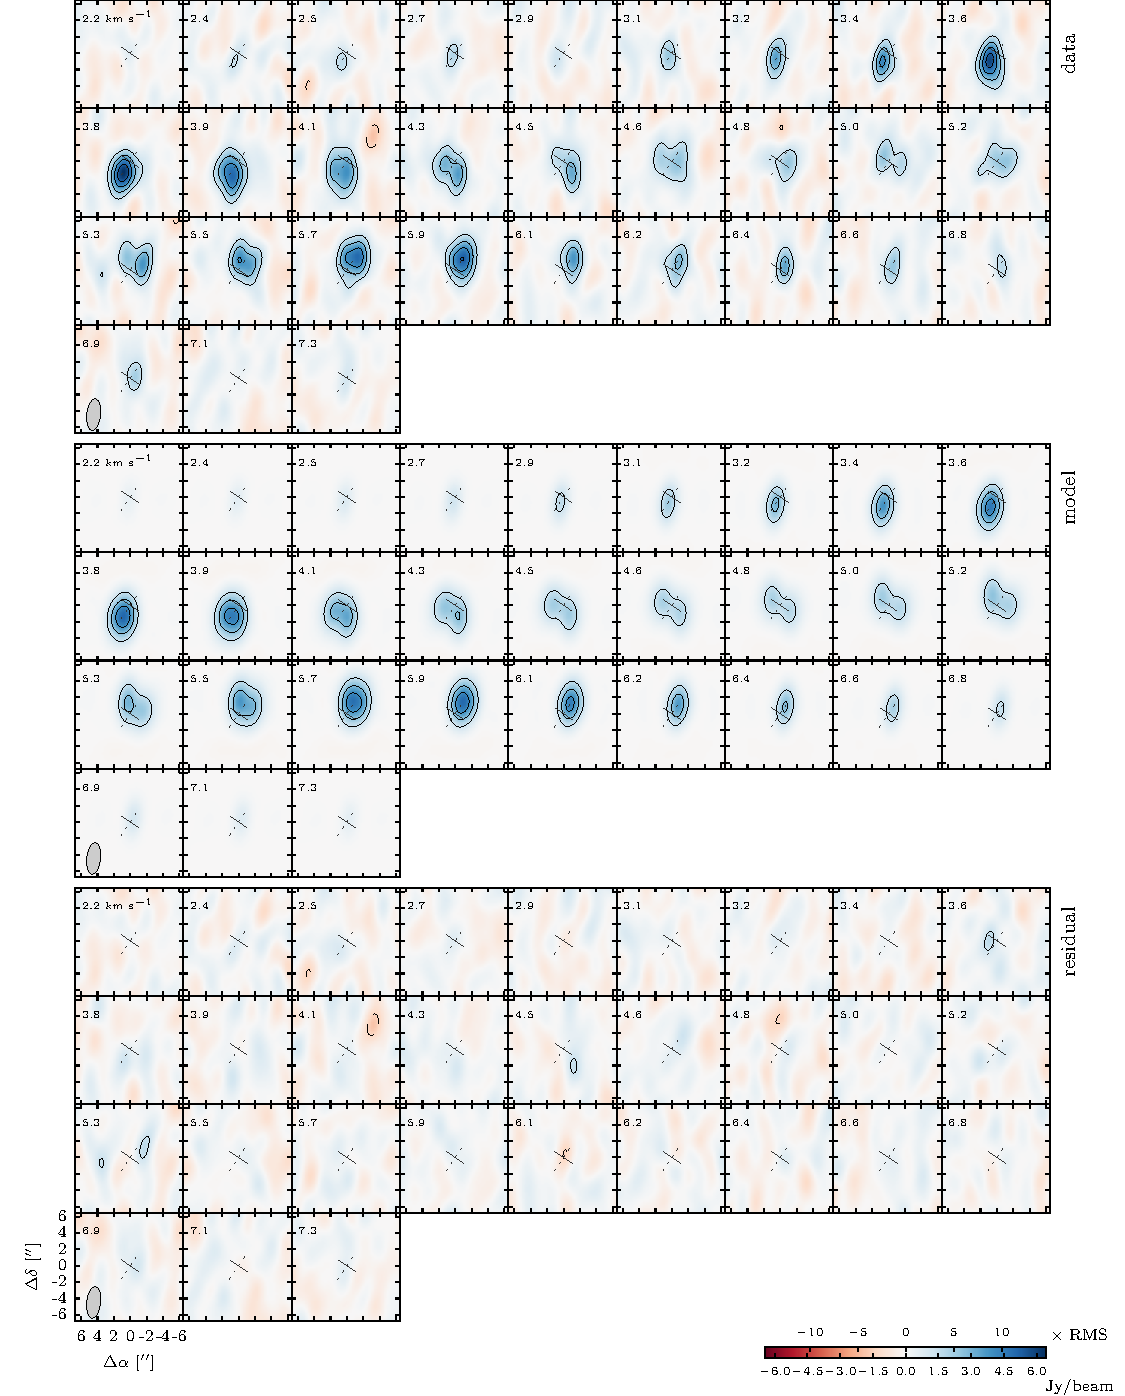
\includegraphics{RXJ1615.pdf}
  \figcaption{
  Same as above, for RX J1615.3-3255.
  \label{fig:RXJ1615}}
  \end{center}
\end{figure*}

\citep{vandermarel15} derives PA = 153, i = 45, vsrc = 4.6 km/s. Says no dust cavity visible. Andrews 11 has cavity of 30 AU.

Large range of permissible CO densities inside gap before CO makes optically thick-thin transition.

\citep{andrews11}
Wichmann et al 1997

Spt = K5

$M = 1.1 M_\odot$.
d = 185 pc.

\subsection{RX J1633.9-2442}

\begin{figure*}[htb]
\begin{center}
  \includegraphics[draft, width=0.95\textwidth, height=5in]{RXJ1633.pdf}
  \figcaption{
  Same as above, for RX J1633.9-2442.
  \label{fig:RXJ1633}}
  \end{center}
\end{figure*}

\subsection{AS 209}

% van Leeuwen 07 parallax
% 7.63 [2.91]

% 95
% 131
% 212

\begin{figure*}[htb]
\begin{center}
  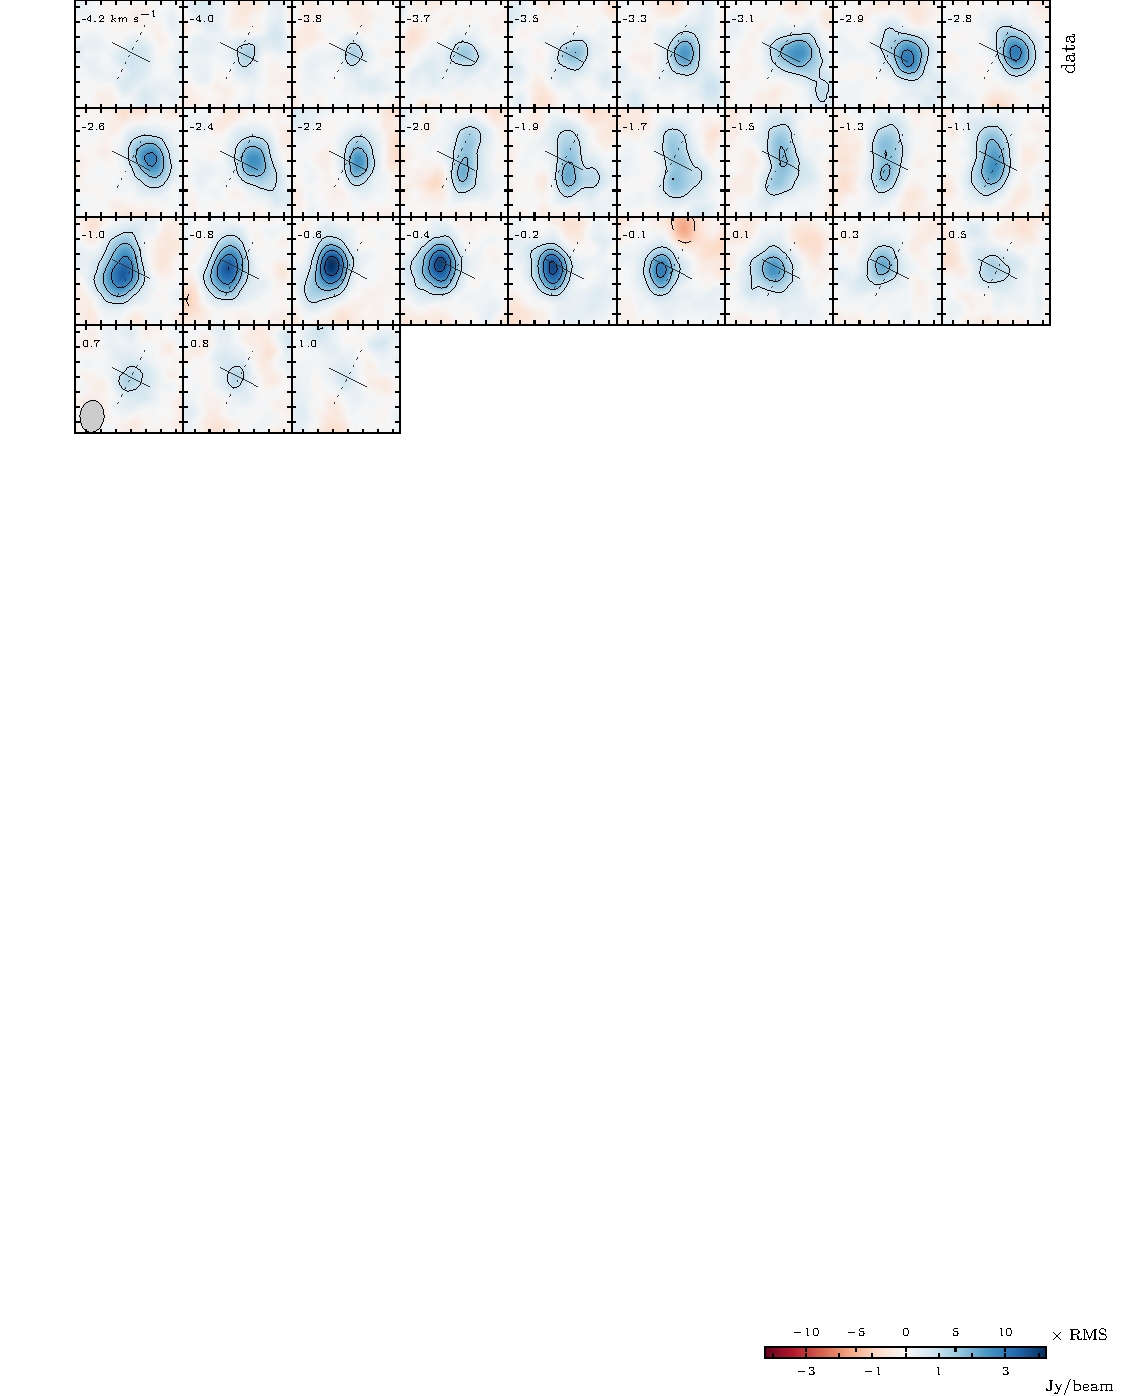
\includegraphics{AS209.pdf}
  \figcaption{
  Same as above, for AS~209.
  \label{fig:AS209}}
  \end{center}
\end{figure*}

Mask central channels due to cloud contamination.

\subsection{HD 163296}

\begin{figure*}[htb]
\begin{center}
  \includegraphics[draft, width=0.95\textwidth, height=5in]{HD163296.pdf}
  \figcaption{
  Same as above, for HD~163296.
  \label{fig:HD163296}}
  \end{center}
\end{figure*}

\subsection{HD 169142}

\begin{figure*}[htb]
\begin{center}
  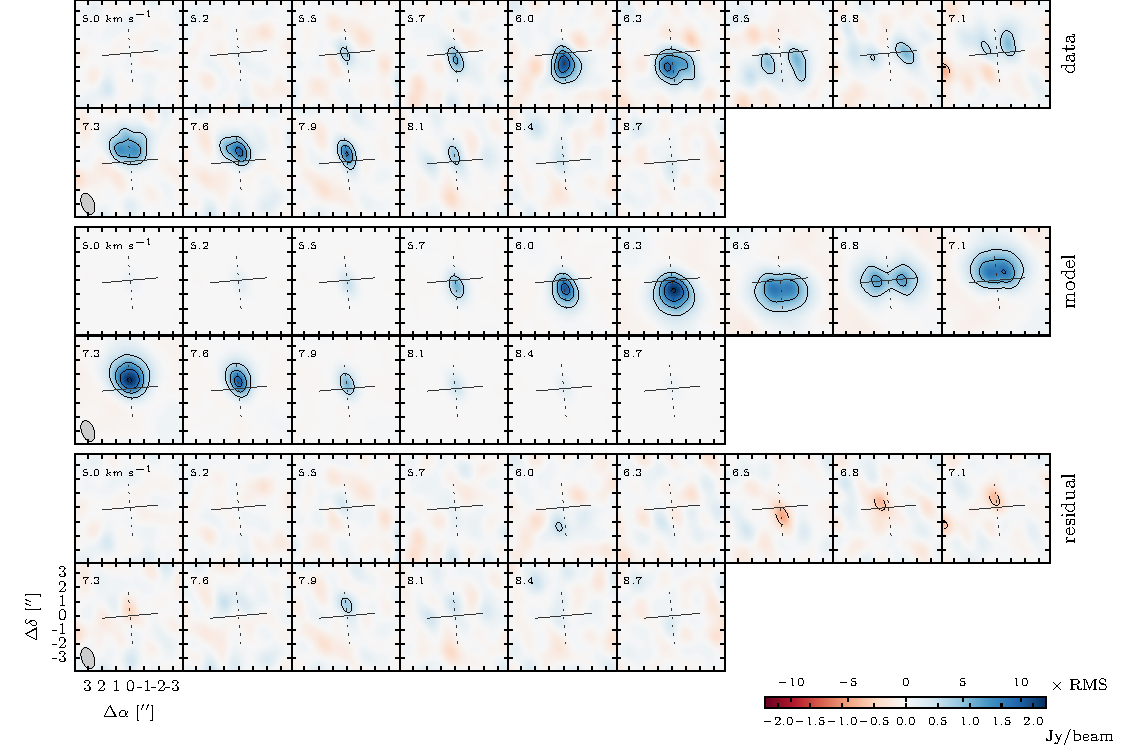
\includegraphics{HD169142.pdf}
  \figcaption{
  Same as above, for HD~169142.
  \label{fig:HD169142}}
  \end{center}
\end{figure*}

Fit with both standard and cavity models.

Appears to be a definite inner cavity in the gas.

\end{document}
